%results 05-21 10-39.mat
\subsection{Badania przesiewowe dla małej ilości neuronów}
Celem pierwszego eksperymentu było zbadanie, jaki wpływ na poprawność klasyfikacji i błąd średnio-kwadratowy ma mała liczba neuronów. W pętlach kolejno zmieniana była ilość neuronów w obu warstwach, w zakresie od 1 do 10 z krokiem 1, a następnie na podstawie uzyskanych w obliczeniach danych zostały utworzone potrzebne wykresy (listing (\ref{skrypt})).Wartości pozostałych parametrów zostały ustawione na domyślne tj. wartość współczynnika inkrementacji na $1.05$, wartość współczynnika dekrementacji na $0.7$, dopuszczalna krotność przyrostu błędu na $1.04$.

\begin{figure}[!h]
\centering
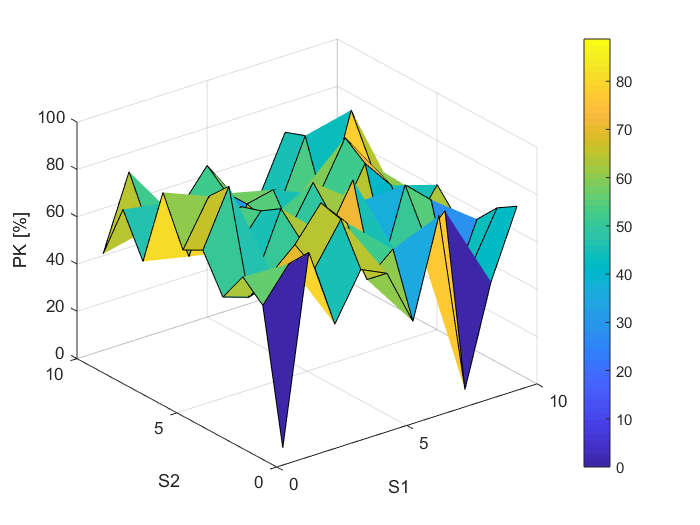
\includegraphics[width = 0.7\textwidth]{Grafika/przesiewowe_male.png}
\caption{Wpływ liczby neuronów w warstwie pierwszej i drugiej na poprawność klasyfikacji}
\label{fig:PKeksperyment1}
\end{figure}
\begin{figure}[!h]
\centering
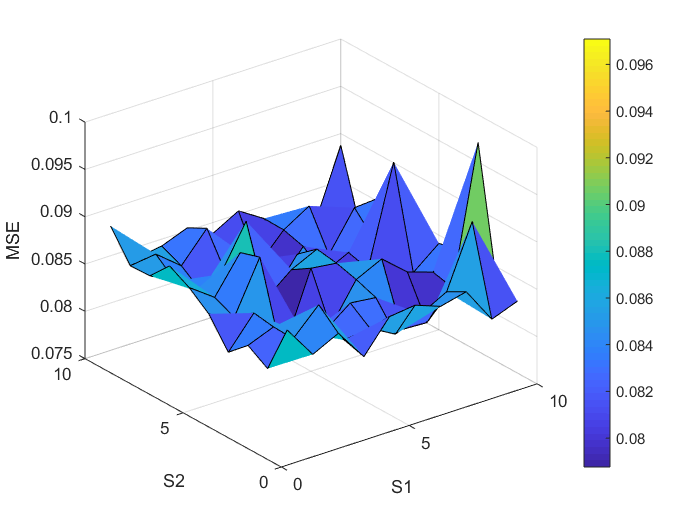
\includegraphics[width = 0.7\textwidth]{Grafika/mse_przesiewoweMale.png}
\caption{Wpływ liczby neuronów w warstwie pierwszej i drugiej na błąd średnio-kwadratowy}
\label{fig:MSEeksperyment1}
\end{figure}
\clearpage
Największą poprawność klasyfikacji ($88.75\%$) uzyskano dla 2 neuronów w warstwie pierwszej i 5 w warstwie drugiej.\\
Najmniejszy błąd średnio-kwadratowy ($0.0795748$) osiągnięty został dla 8 neuronów w warstwie pierwszej i 10 neuronów w warstwie drugiej. Dla tej konfiguracji $PK$ wyniosło $67.63\%$.




